\documentclass[11pt, pdflatex, compress]{beamer}
\mode<presentation>
\useoutertheme{tree}
\setbeamercolor{separation line}{use=structure,bg=structure.fg!50!bg}
\usetheme[progressbar=foot, numbering=none]{metropolis}

\hypersetup{pdfpagemode=FullScreen}
\usepackage[english]{babel}
\usepackage[T1]{fontenc}
\usepackage[latin1]{inputenc}
%% \usepackage[sfdefault]{FiraSans}


\usepackage{amsmath, amssymb, amsthm} 
	   % accents dans le pdf

%\EnableBpAbbreviations 
\usepackage{xcolor}
%\RequirePackage[cmyk]{xcolor}

\linespread{1.2}
\usepackage{graphics,graphicx,subfigure}
\usepackage{comment}
\usepackage{float} 
\usepackage{xcolor}
\usepackage{framed}
\usepackage{multicol}

\makeatletter
\setlength{\metropolis@progressinheadfoot@linewidth}{1.5pt}
\setlength{\metropolis@progressonsectionpage@linewidth}{1.5pt}
\makeatother

% config text
\setlength\textwidth{10cm}          % largeur du texte
%% \setlength\topmargin{-3cm}          % marge en haut     % marge de gauche
\setlength\textheight{24cm}         % hauteur du texte
\setlength\oddsidemargin{\evensidemargin}
\usepackage{fancybox}
\usepackage{graphicx}
\usepackage{mathpazo}
\usepackage{mdframed}
\usepackage{booktabs}
 

%%%%%



\usepackage{color,transparent}
%%%%%

\definecolor{bordercol}{gray}{0.95}
%\definecolor{headercol1}{RGB}{186,215,230}
\definecolor{col1}{RGB}{186,225,230}
\definecolor{col2}{RGB}{120,150,120}
\definecolor{header}{RGB}{0,0,0}
\definecolor{boxy}{cmyk}{0,0.01,0.05,0}
\definecolor{back}{RGB}{11,11,70}
\definecolor{BlueViolet}{RGB}{120,40,120}
\setbeamercolor{background canvas}{bg=white}



\begin{document}


   	\title{
\includegraphics[scale=0.10]{logoincc.jpg}  
\includegraphics[scale=0.3]{ed3c.png} 
\includegraphics[scale=0.05]{logouniv.jpg}  
\includegraphics[scale=0.03]{logocnrs.png} \\
      
 {\textcolor{back}{Eureka moments in the acquisition of mathematical concepts}}\\
        {\small {\textcolor{back}{Charlotte Barot, Louise Chevalier, Lucie Martin and  V\'{e}ronique Izard }}}\\
        
        }

        



        




     \begin{frame}
      \titlepage
     \end{frame}


           


\small
\section{Introduction}


\subsection{Context and motivation}

\begin{frame}

\centering
How does it feel to understand a mathematical concept ?

\end{frame}

\begin{frame}




Famous scientists experience sudden \textcolor{orange}{``Eureka moments''}, notably in mathematics (Poincar\'{e} 1908, Hadamard 1959)

 \textcolor{orange}{Sudden and unexpected understanding}
 \textcolor{orange}{Feeling of certainty}



\end{frame}


\begin{frame}



 Famous scientists experience sudden \textcolor{orange}{``Eureka moments''}, notably in mathematics (Poincar\'{e} 1908, Hadamard 1959)

      \textcolor{orange}{Sudden and unexpected understanding}
     \textcolor{orange}{Feeling of certainty}
  

\ite Similar experiences are studied in the scope of problem solving where \textcolor{orange}{solutions} come by ``insight''

\en

  
\end{frame}




\bef\tif{  Context and motivation}



\be
\ite Famous scientists experience sudden \textcolor{orange}{``Eureka moments''}, notably in mathematics (Poincar\'{e} 1908, Hadamard 1959)
   \be
     \ite \textcolor{orange}{Sudden and unexpected understanding}
     \ite \textcolor{orange}{Feeling of certainty}
   \en

\ite Similar experiences are studied in the scope of problem solving where \textcolor{orange}{solutions} come by ``insight''
    \be
   \ite \textcolor{orange}{No awareness that it was about to come }
   \ite \textcolor{orange}{Immediately perceived as correct and relevant }
  \en


\en

  
\end{frame}


\bef\tif{  Context and motivation}



\be
\ite Famous scientists experience sudden \textcolor{orange}{``Eureka moments''}, notably in mathematics (Poincar\'{e} 1908, Hadamard 1959)
   \be
     \ite \textcolor{orange}{Sudden and unexpected understanding}
     \ite \textcolor{orange}{Feeling of certainty}
   \en

\ite Similar experiences are studied in the scope of problem solving where \textcolor{orange}{solutions} come by ``insight''
 \be
   \ite \textcolor{orange}{No awareness that it was about to come }
   \ite \textcolor{orange}{Immediately perceived as correct and relevant }
  \en
\en

\centering

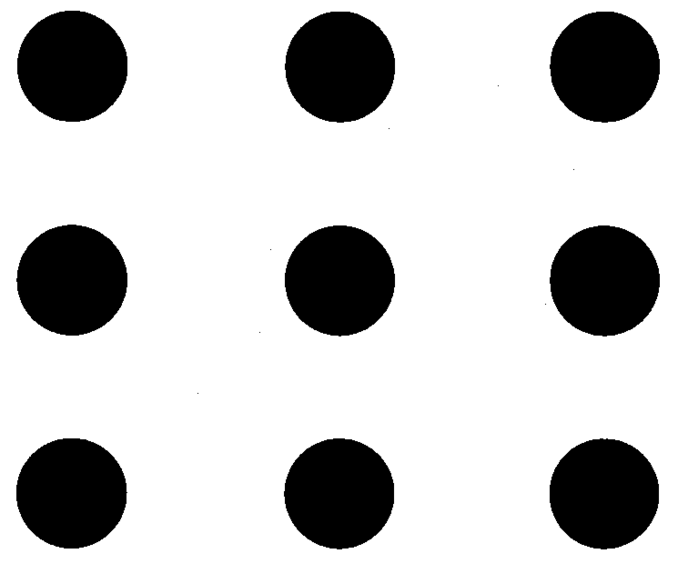
\includegraphics[scale=0.10]{nine.png}

\footnotesize{The nine dot problem, Lung and  Dominowski 1985}
  
\end{frame}

  
\subsection{Main question} 



\bef
So far, no evidence of insights while learning a new  concept
\bigskip

\centering

\includegraphics[scale=0.8]{maggie_maths.png}
\end{frame}


\bef \tif{Methodological difficulties}
Learning science concepts is difficult and protracted (Carey 2009,Weber 2002, Asmuth and Rips 2006, Vosniadou 2019)

\be

\ite Conducted in classrooms (Cross sectional designs or longitudinal designs with long delays between sessions)
\ite Lab experiment with simple learning targets  (Ohlsson 2009) for example inferring a rule for categorizing images
\en
\end{frame}





\subsection{Goals of the study}
\bef

\be \tif{Goals}
\ite Conceive a one session paradigm of conceptual learning, to access participants objective and subjective progress and modulate level of understanding through conditions 
\ite See if participants report experiencing insights while learning a new concept and if these insights are related to performance
\ite Evaluate the relation between experiences of insights and other forms of introspection in a concept learning context 
\en

\end{frame}

 

\section{Material and Methods}



\subsection{Learning situation}


\subsection{Learning situation}




\bef \tif{The new concept : geodesic}
Geodesic is the generalization of straight line to curved surfaces

Starting from a given point on a surface, it is a path which has a constant direction and never turns

\end{frame}





\bef \tif{Learning situation : geodesic on the sphere}

\centering
"Is it straight?"

\begin{tabular}{cccc}
  
\ig[scale=0.2]{co.png} & \ig[scale=0.2]{gc.png} & \ig[scale=0.2]{pc.png} \\

        &   &   \\

\end{tabular}

 \end{frame}




\bef \tif{Learning situation : geodesic on the sphere}

\centering
"Is it straight?"

\begin{tabular}{cccc}
  
\ig[scale=0.2]{co.png} & \ig[scale=0.2]{gc.png} & \ig[scale=0.2]{pc.png} \\

\ig[scale=0.4]{nein.png} &   &   \\

\end{tabular}
\end{frame}


\bef \tif{Learning situation : geodesic on the sphere}

\centering
"Is it straight?"

\begin{tabular}{cccc}
  
\ig[scale=0.2]{co.png} & \ig[scale=0.2]{gc.png} & \ig[scale=0.2]{pc.png} \\

\ig[scale=0.4]{nein.png} &  \ig[scale=0.4]{checky.png} &   \\

\end{tabular}

 \end{frame}





\bef \tif{Learning situation : geodesic on the sphere}



\centering
"Is it straight?"

\begin{tabular}{cccc}
  
\ig[scale=0.2]{co.png} & \ig[scale=0.2]{gc.png} & \ig[scale=0.2]{pc.png} \\

\ig[scale=0.4]{nein.png} &  \ig[scale=0.4]{checky.png} &   \ig[scale=0.4]{nein.png} \\

\end{tabular}

 \end{frame}




\bef \tif{Learning phase  \hspace*{3cm}}

\ig[scale=0.85]{learningy.png}

\centering
The rubber band lesson

 \ig[scale=0.16]{elastoc.jpg}  \ig[scale=0.04]{elastoc1.jpg}  \ig[scale=0.04]{elastoc2.jpg}

\tiny{ The elastic is straight and follows greater circles on
   a sphere, but when applied to a small circle, the elastic does not follow the line }

\bigskip

Four conditions : 1, 3, 5 or 7 different lessons
 \end{frame}




\bef \tif {Experimental protocol}

\centering
\ig[scale=0.99]{protoc.png}

\tiny{N=56, 18-43 years (\it M=25.5),
time $ \thickapprox $ 1h30}
\end{frame}




\bef \tif {Preliminary tests}

\ig[scale=0.27]{pretesty.pdf}

\centering

\ig[scale=0.22]{ligne.png}

\centering
\ig[scale=0.02]{cot}  \ig[scale=0.02]{gct}   \ig[scale=0.02]{pct}

\end{frame}




\subsection{Performance measures}

\bef \tif {Performance measures : Test1}

\ig[scale=0.85]{test1y.png}
  
\centering

\begin{tabular}{cccc}

\ig[scale=0.02]{cot} &   \ig[scale=0.02]{gct} &  \ig[scale=0.02]{pct}  \\

\tiny{Not straight non planar lines} & \tiny {Straight planar lines} & \tiny{Not straight planar lines} \\

\end{tabular}

\end{frame}





\bef \tif {Performance measures: Test2 }

 \ig[scale=0.85]{protoct2.png}

\centering

\begin{tabular}{cccc}

  \ig[scale=0.3]{conenf.png} &   \ig[scale=0.3]{coneof.png} &  \ig[scale=0.3]{conend.png} &  \ig[scale=0.3]{coneod} \\
                               &  &  &   \\

                               &   &  &  \\

\end{tabular}
\end{frame}





\bef \tif {Performance measures: Test2 }

 \ig[scale=0.85]{protoct2.png}

\centering

\begin{tabular}{cccc}

   \ig[scale=0.3]{conenf.png} &   \ig[scale=0.3]{coneof.png} &  \ig[scale=0.3]{conend.png} &  \ig[scale=0.3]{coneod.png} \\

      \ig[scale=0.2]{nein.png} &  &  &   \\

 \tiny{Non straight non planar lines} &   &  &  \\

\end{tabular}
\end{frame}




\bef \tif {Performance measures: Test2 }

 \ig[scale=0.85]{protoct2.png}

\centering

\begin{tabular}{cccc}

   \ig[scale=0.3]{conenf.png} &   \ig[scale=0.3]{coneof.png} &  \ig[scale=0.3]{conend.png} &  \ig[scale=0.3]{coneod.png} \\

      \ig[scale=0.2]{nein.png} &  \ig[scale=0.2]{checky.png} &  &   \\

 \tiny{Non straight non planar lines} &  \tiny{Straight planar lines} &  &  \\

\end{tabular}
\end{frame}




\bef \tif {Performance measures: Test2 }

 \ig[scale=0.85]{protoct2.png}

\centering

\begin{tabular}{cccc}

   \ig[scale=0.3]{conenf.png} &   \ig[scale=0.3]{coneof.png} &  \ig[scale=0.3]{conend.png} &  \ig[scale=0.3]{coneod.png} \\

      \ig[scale=0.2]{nein.png} &  \ig[scale=0.2]{checky.png} &  \ig[scale=0.2]{nein.png} &   \\

 \tiny{Non straight non planar lines} &  \tiny{Straight planar lines} &  \tiny{Not  straight planar lines} &  \\

\end{tabular}
\end{frame}


\bef \tif {Performance measures: Test2 }

 \ig[scale=0.85]{protoct2.png}

\centering

\begin{tabular}{cccc}

   \ig[scale=0.3]{conenf.png} &   \ig[scale=0.3]{coneof.png} &  \ig[scale=0.3]{conend.png} &  \ig[scale=0.3]{coneod.png} \\

      \ig[scale=0.2]{nein.png} &  \ig[scale=0.2]{checky.png} &  \ig[scale=0.2]{nein.png} & \ig[scale=0.2]{checky.png}  \\

 \tiny{Non straight non planar lines} &  \tiny{Straight planar lines} &  \tiny{Not  straight planar lines} & \tiny{Straight non planar lines} \\

\end{tabular}
\end{frame}
 

 


\bef \tif {Performance measures: Test3}

 \ig[scale=0.85]{protoct3.png}

\centering

\tiny{Test condition Sphere}

\ig[scale=0.8]{testy3.pdf}

\tiny{Test condition All surfaces}

\ig[scale=0.8]{surface.pdf}



\end{frame}



\subsection{introspection measures}

\bef \tif{Introspection measures }

 \ig[scale=0.85]{introy.png}

 \be

\ite Feeling Of Understading (FOU)  rating from 0 to 10

\centering
\ig[scale=0.17]{intro.png}

 \ite Insight reports ``Did you experienced an insight ?''

\tiny{(description adapted from Danek and Wiley 2017)}


\en


\end{frame}

\section{Analyses}

\bef

\be

\ite Is performance influenced  by the number of lessons ?

\ite Do participants report insights ?

\ite Are insights related to a good performance ?

\ite What is the relation between insight reports and feelings of knowing ?

\en

\end{frame}


\section{Results}


\section{Is performance influenced by the number of lessons ?}



\bef \tif{Is performance influenced by the number of lessons ? first test}

\centering

\ig[scale=0.4]{test1_cond.pdf}
\tiny{ \it Predictions of the logistic mixed model by test condition and number of lessons, with individual participants' performance, corrected for years of mathematic education after 10th grade} 

 \tiny{N=56, 18-43 years (\it M=25.5)}

\end{frame}


\bef \tif{Is performance influenced by the number of lessons ? Second test}

 \centering
 \ig[scale=0.4]{test2_cond.pdf}

 \tiny{N=56, 18-43 years (\it M=25.5)}
\end{frame}


\bef \tif{Is performance influenced by the number of lessons ? Third test}
  \centering
 \ig[scale=0.4]{test3_cond.pdf}

 \tiny{N=56, 18-43 years (\it M=25.5)}
\end{frame}



\bef \tif{Is FOU influenced by the number of lessons ? }
 \centering
 \ig[scale=0.4]{intro_cond1.pdf}

 \tiny{\it Predictions of the mixed model by measurement time and number of lessons, with individual participants feeling of knowing, corrected for years of mathematic education after 10th grade

  Feeling of understanding 1:  measured just after participants completed the teaching phase; Feeling of understanding 2: measured after the various surfaces straight lines test;
  Feeling of understanding 3:
  measured after the reasoning test} 

 \tiny{N=56, 18-43 years (\it M=25.5)}


\end{frame}

\section{Did participants report insights and are these insights related to a good performance ?}



\bef \tif{Insight reports}

  60 \% of insight reports, more insights reported in the conditions with more lessons (**)

  \centering
  \ig[scale=0.4]{ins_cond.pdf}

  \tiny{\it Predictions of the binomial linear model by number of lessons, with individual participants' insight reports, corrected for years of mathematic education after 10th grade} 

  \tiny{N=56, 18-43 years (\it M=25.5)}

\end{frame}


\section{What is the relation between the different introspection measures ?}


\bef \tif{Relations between introspection measures}
 \begin{table}

	\label{tab:schemes}
	\centering
	\begin{tabular}{ccccc}
		 \toprule
  \tiny Introspection measure	& \tiny FOU 1		& \tiny FOU 2		        & \tiny FOU 3		& \tiny Insight\\

		 \midrule
	\tiny 	FOU 1     	& \tiny X		& \tiny .6 (<.0001)		& \tiny .6 (<.0001)	& \tiny .27 (.13) \\
	\tiny	FOU 2    	& \tiny .6 (<.0001)	& \tiny X     		        & \tiny .85 (.<0001)	& \tiny .19 (.33)\\
	\tiny	FOU 3    	& \tiny .6 (<.0001)	& \tiny .85 (<.0001)		& \tiny X		& \tiny .17 (.33) \\
	\tiny	Insight       	& \tiny .15 (.81)	& \tiny .14 (.81) 		& \tiny .15 (.81)	& \tiny X          \\
		\bottomrule
	\end{tabular}
 \end{table}

 \tiny{Spearman's rho coefficients and p values for pairwise correlation tests. Above diagonal : zero-order correlation, below: with number of lessons and education in mathematics as covariates.
     All p values were corrected for multiple comparisons using Holm's  method.

     Feeling of understanding 1:  measured just after participants completed the teaching phase; Feeling of understanding 2: measured after the various surfaces straight lines test;
     Feeling of understanding 3:
  measured after the reasoning test.}
\end{frame}




\bef \tif{Relations between generalization test condition and introspection measures}
\centering
\ig[scale=0.6]{difoui.pdf}

\tiny{\it Predictions of the logistic mixed model by number of lessons, mean introspection and insight reports, with individual participants' performance, corrected for years of mathematic education after 10th grade} 

\tiny{N=56, 18-43 years (\it M=25.5)}
\end {frame}





\section{Conclusion}

\bef \tif{Overview of results}
Participants learned and they learned a concept

  \be
   \ite Reading more lessons led to better performance in several  post-teaching test conditions
   \ite Two characteristic signatures of conceptual learning
   \be
     \ite First, learning was difficult (cf positive linear effects of the number of lessons on test performance, accounting that all lessons had the same  maths content)
     \ite Content learned was inferentially rich (ability to draw inferences from this information)

     Non trivial inferences about the properties of straight lines in spherical geometry : realize that two straight lines drawn on a sphere can never be parallel
     \en
   \en

\end{frame}

\bef{Overview of results}

 Participants reported insights and these insights are related to the learning process
\be
  \ite After reading this description, a little over half of our participants reported experiencing insight episodes during the course of our experiment (60\%)

  \ite Modulated by our experimental manipulation and consistent with performance. (not simply reflect variations in the personalities,
  or in level in mathematics)
  \ite  Relation between insights and performance
  took the form of an interaction (insights related to better performance in some but not all test conditions), even when controlling for number of lessons, level in maths, and FOU
   

 \en
\end{frame}


\bef
Insights and introspection are dissociated, and only insights are related to learning
in a test of generalization for their new concept of straight line

 \be
 \ite  FOU measures strongly correlated  but none was correlated to experiences of insight
 
 \ite Insight experiences uniquely associated with performance in one of our test condition, even after controlling for FOU

     \centering

     \ig[scale=0.3]{coneod}
   
  
   \ite FOU was also related to post-teaching performance independently of the presence of insights (relation is difficult to decipher as the ratings of FOU did not map any test condition)
  \en


\end{frame}


\bef \tif{Discussion}
 Do the insights experienced during concept learning and during problem solving reflect similar psychological mechanisms? 
 \be
  \ite Insight vs confidence
 \en
\end{frame}

\bef \tif{Discussion}
  Do the insights experienced during concept learning and during problem solving reflect similar psychological mechanisms? 
  \be
   \ite Insight vs confidence
   \ite Insight and representational change
  \en
\end{frame}



\bef \tif{Discussion}
  Do the insights experienced during concept learning and during problem solving reflect similar psychological mechanisms? 
  \be
   \ite Insight vs confidence  
   \ite Insight and  representational change 
   \ite Continuous vs discrete %% : do insights indicate crucious steps of uncounscious learning process?
   \en
\end{frame}



\bef{Discussion}
  Is concept learning subtended by a cumulative process?
\end{frame}

\bef[standout]
\centering
Thanks for your attention  !
\end{frame}

\end{document}
